\section{La función de nutrición}

Mediante la función de nutrición, tomamos alimentos y agua, respiramos oxígeno, utilizamos estas sustancias para vivir y crecer, y expulsamos los desechos.

\vspace{3mm}
Para realizar esta función, trabajan coordinadamente cuatro aparatos: el \textbf{digestivo}, el \textbf{respiratorio}, el \textbf{circulatorio} y el \textbf{excretor}.

\subsection{Los nutrientes y los alimentos}

\subsubsection{Los nutrientes}

Los nutrientes son todas aquellas sustancias que obtenemos de los alimentos y que necesitan las células de nuestro cuerpo para realizar sus funciones vitales. Los principales nutrientes son:

\begin{itemize}
    \item Los \textbf{hidratos de carbono} o azúcares proporcionan energía.
    \item Los \textbf{lípidos} pueden ser de distintos tipos, y cumplen diversas funciones. Por ejemplo, las grasas proporcionan energía; pueden ser almacenadas en algunas células de la piel como una reserva energética que, además, nos aísla del frío.
    \item Las \textbf{proteínas} son imprescindibles para que las células se formen, crezcan y desarrollen tejidos.
    \item Las \textbf{vitaminas} y las \textbf{sales minerales} regulan el funcionamiento general del organismo.
    \item El \textbf{agua} constituye la mayor parte del contenido de las células, de la sangre, etc. Sin ella, no funcionaría el organismo.
\end{itemize}

\subsubsection{Los alimentos}

Según los nutrientes que contienen, los alimentos se clasifican en energéticos, constructivos y reguladores.

\begin{itemize}
    \item Los \textbf{alimentos energéticos} contienen hidratos de carbono o grasas. Son los aceites vegetales, las grasas animales, la mantequilla, las patatas y los cereales y sus derivados, como las pastas, los dulces y el pan.
    \item Los \textbf{alimentos constructivos} contienen proteínas. Son las legumbres, las carnes de animales terrestres o marinos, los huevos y la leche y sus derivados, como los yogures y los quesos.
    \item Los \textbf{alimentos reguladores} contienen vitaminas y sales minerales. Son las verduras, las hortalizas y las frutas.
\end{itemize}

\subsubsection{La dieta y la rueda de los alimentos}

La \textbf{dieta} es el conjunto de los alimentos y el agua que toma cada día una persona. La \textbf{dieta es saludable} cuando contiene una cantidad adecuada de cada uno de los nutrientes.

\vspace{3mm}
Para que resulte más fácil elaborar dietas saludables, los alimentos se representan en la \textbf{rueda de los alimentos} (Figura \ref{fig:rueda-alimentos}), un gráfico que nos orienta sobre la frecuencia con la que se deben consumir los diferentes alimentos.

\begin{figure}[!ht]
    \centering
    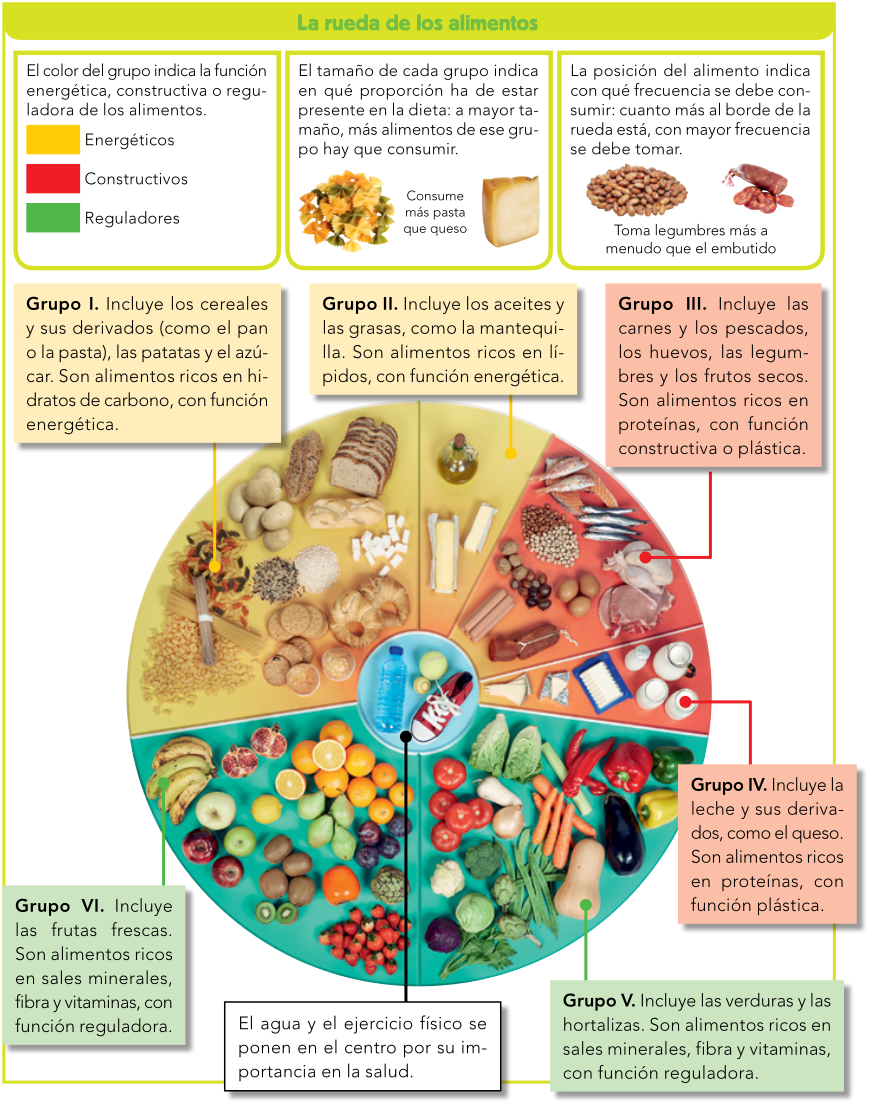
\includegraphics[width=1\linewidth]{Tema3/01_Rueda_alimentos.png}
    \caption{Rueda de los alimentos}
    \label{fig:rueda-alimentos}
\end{figure}

\subsection{El aparato digestivo y la digestión}

Nuestras células necesitan nutrientes y agua para llevar a cabo sus actividades. Estas sustancias las obtenemos de los alimentos y las bebidas mediante la digestión. El aparato encargado de realizar la digestión es el aparato digestivo (Figura \ref{fig:aparato-digestivo}).

\subsubsection{Cómo es el aparato digestivo}

El aparato digestivo está formado por el tubo digestivo y las glándulas anejas.

\begin{itemize}
    \item El \textbf{tubo digestivo} es un largo conducto compuesto por la boca, la faringe, el esófago, el estómago, el intestino delgado, el intestino grueso y el ano.
    \item Las \textbf{glándulas anejas} son órganos que se encuentran fuera del tubo digestivo pero que vierten en él las sustancias que producen. Son las \textbf{glándulas salivales}, el \textbf{hígado} y el \textbf{páncreas}.
\end{itemize}

\begin{figure}[!ht]
    \centering
    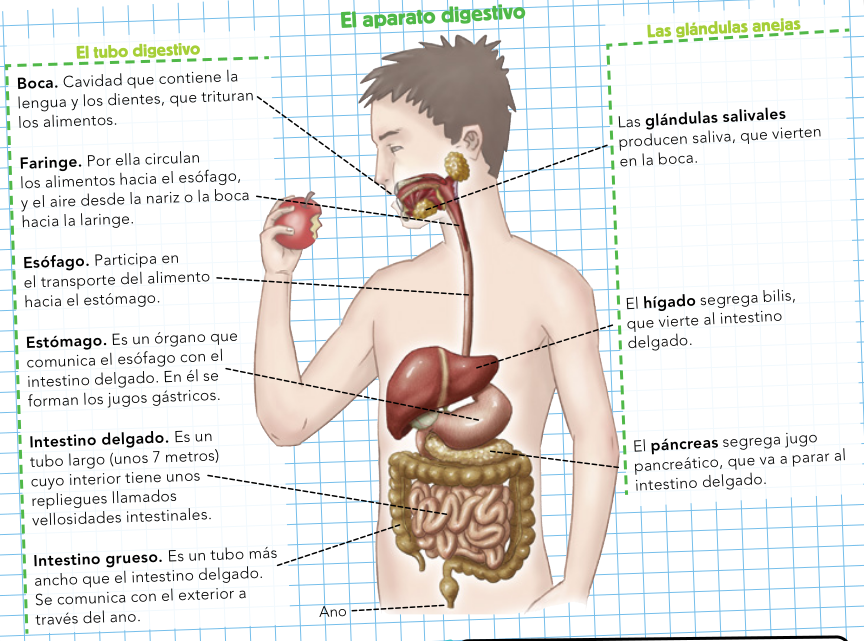
\includegraphics[width=0.8\linewidth]{Tema3/02_Aparato_digestivo.png}
    \caption{El aparato digestivo}
    \label{fig:aparato-digestivo}
\end{figure}

\subsubsection{La digestión}

La \textbf{digestión} (Figura \ref{fig:digestion}) es la transformación de los alimentos que tomamos, para extraer de ellos los nutrientes. Tiene lugar a lo largo del tubo digestivo, y se lleva a cabo en varias etapas.

\vspace{3mm}
\textbf{En la boca}

\vspace{3mm}
En la boca, los dientes y las muelas cortan y trituran los alimentos. Estos se mezclan con la saliva, gracias a los movimientos de la lengua, y se forma el \textbf{bolo alimenticio}. Este, al ser tragado, baja por la faringe y el esófago hasta el estómago.

\vspace{3mm}
\textbf{En el estómago}

\vspace{3mm}
Cuando llega el bolo alimenticio al estómago, sus paredes segregan unas sustancias, los jugos gástricos, que digieren parcialmente el alimento y lo transforman en una papilla, llamada \textbf{quimo}.

\vspace{3mm}
\textbf{En el intestino delgado}

\vspace{3mm}
Cuando el quimo llega al intestino delgado, se vierten en él el jugo pancreático (procedente del páncreas) y la bilis (procedente del hígado). Se completa así la digestión de los alimentos y el quimo se transforma en el \textbf{quilo}.

\vspace{3mm}
A continuación, los nutrientes del quilo pasan a la sangre a través de los capilares que se encuentran en el intestino delgado, este proceso se llama \textbf{absorción}.

\vspace{3mm}
\textbf{En el intestino grueso}

\vspace{3mm}
El agua y los desechos pasan al intestino grueso. Allí se reabsorbe el agua de la mezcla y se forman las \textbf{heces}, sustancias de desecho que son expulsadas por el ano.

\begin{figure}[!ht]
    \centering
    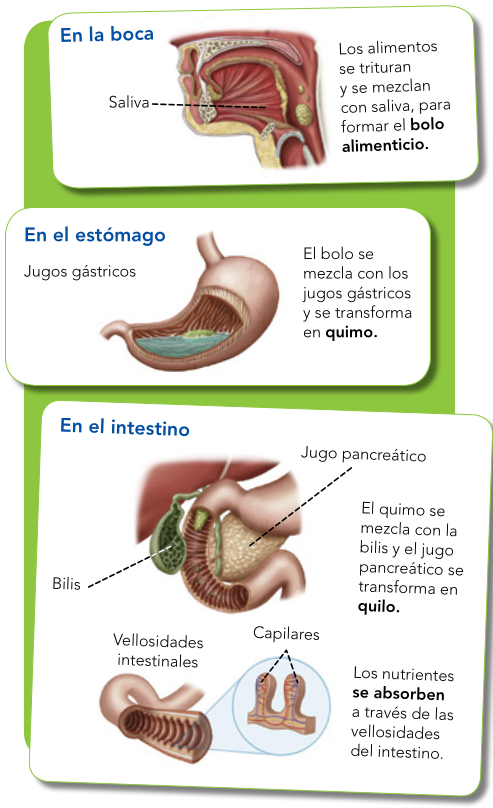
\includegraphics[width=0.7\linewidth]{Tema3/03_Digestion.png}
    \caption{La digestión}
    \label{fig:digestion}
\end{figure}

\subsection{El aparato respiratorio y la respiración}

\subsubsection{Las células necesitan oxígeno}

Mediante la respiración, obtenemos del aire el oxígeno que necesitan nuestras células y expulsamos al exterior el dióxido de carbono que estas producen como desecho. De este proceso se encarga el aparato respiratorio.

\subsubsection{El aparato respiratorio}

El aparato respiratorio (Figura \ref{fig:aparato-respiratorio}) está formado por las vías respiratorias y por los pulmones.

\vspace{3mm}
\textbf{Las vías respiratorias}

\vspace{3mm}
Las vías respiratorias son tubos que conectan los pulmones con el exterior. Son las \textbf{fosas nasales}, la \textbf{faringe}, la \textbf{laringe}, la \textbf{tráquea} y los \textbf{bronquios}.

\vspace{3mm}
\textbf{Los pulmones}

\vspace{3mm}
Los pulmones son dos órganos esponjosos situados en el tórax y separados del abdomen por un músculo, el \textbf{diafragma}. Están formados por las ramificaciones de los \textbf{bronquios} y por los \textbf{alvéolos}.

\begin{figure}[!ht]
    \centering
    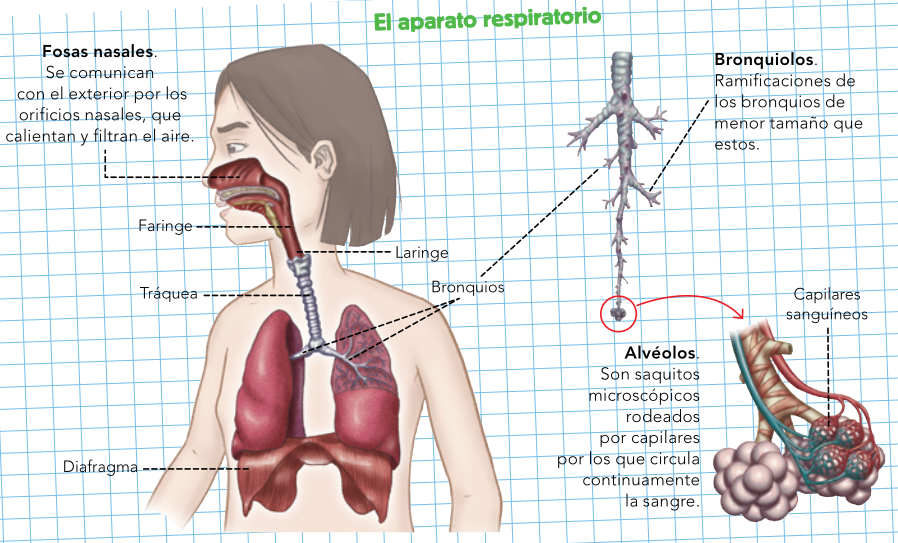
\includegraphics[width=0.9\linewidth]{Tema3/04_Aparato_respiratorio.png}
    \caption{Aparato respiratorio}
    \label{fig:aparato-respiratorio}
\end{figure}

\subsubsection{La respiración}

El aparato respiratorio realiza su función en tres etapas (Figura \ref{fig:respiracion}): la inspiración (o entrada de aire que contiene oxígeno), el intercambio de gases (que sucede en los alvéolos) y la espiración (o expulsión de aire que contiene dióxido de carbono).

\begin{figure}[!ht]
    \centering
    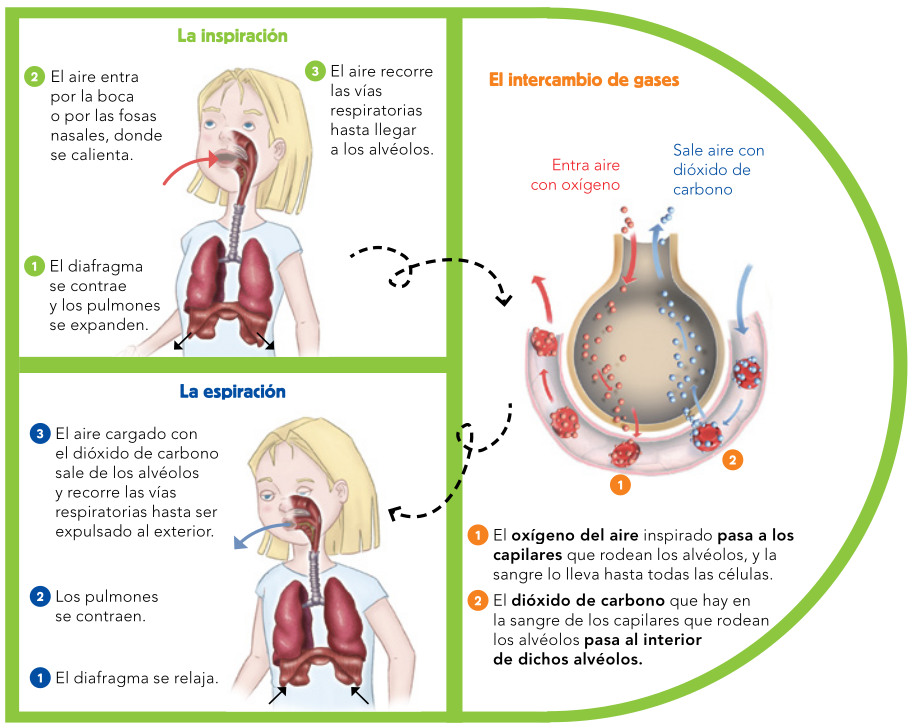
\includegraphics[width=1\linewidth]{Tema3/05_Respiracion.png}
    \caption{La respiración}
    \label{fig:respiracion}
\end{figure}

\subsection{El aparato circulatorio y la circulación}

Las células de nuestro cuerpo necesitan recibir los nutrientes procedentes del aparato digestivo y el oxígeno que llega a través del aparato respiratorio. Además, las células producen desechos, como dióxido de carbono y otras sustancias que hay que llevar hasta los órganos que las eliminan.

\vspace{3mm}
El oxígeno, los nutrientes y los desechos viajan con la sangre de unas partes del cuerpo a otras a través del aparato circulatorio.

\subsubsection{El aparato circulatorio}

El aparato circulatorio está formado por el \textbf{corazón} y por los \textbf{vasos sanguíneos}.

\begin{itemize}
    \item El \textbf{corazón} (Figura \ref{fig:corazon}) es un órgano hueco y musculoso del tamaño de nuestro puño. Está dividido en dos mitades, la izquierda y la derecha, separadas entre sí. En cada mitad hay una cavidad superior, llamada \textbf{aurícula}, y otra inferior, llamada \textbf{ventrículo}; entre ellas hay una \textbf{válvula}, una especie de ``puerta'', que se abre para dejar pasar la sangre en una dirección y se cierra para que esta no vuelva atrás.
    \begin{figure}[!ht]
        \centering
        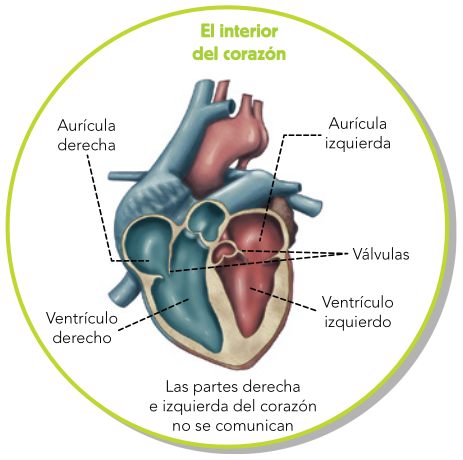
\includegraphics[width=0.6\linewidth]{Tema3/06_Corazon.png}
        \caption{El corazón}
        \label{fig:corazon}
    \end{figure}
    \item Los \textbf{vasos sanguíneos} (Figura \ref{fig:vasos-sanguineos}) son una red de conductos por los que circula la sangre. Son de tres tipos: \textbf{arterias}, \textbf{venas} y \textbf{capilares}.
    \begin{figure}[!ht]
        \centering
        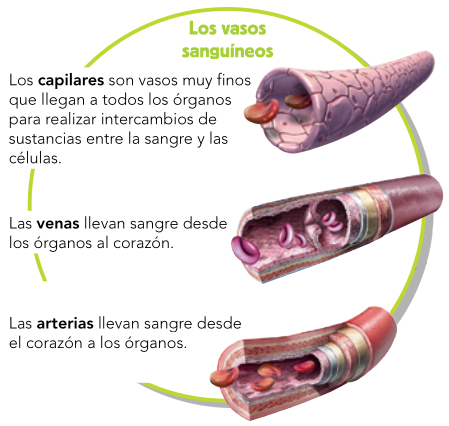
\includegraphics[width=0.7\linewidth]{Tema3/07_Vasos_sanguineos.png}
        \caption{Vasos sanguíneos}
        \label{fig:vasos-sanguineos}
    \end{figure}
\end{itemize}

\subsubsection{La circulación}

La circulación (Figura \ref{fig:circulacion}) se puede dividir en \textbf{circulación pulmonar} y circulación \textbf{general}.

\begin{figure}[!ht]
    \centering
    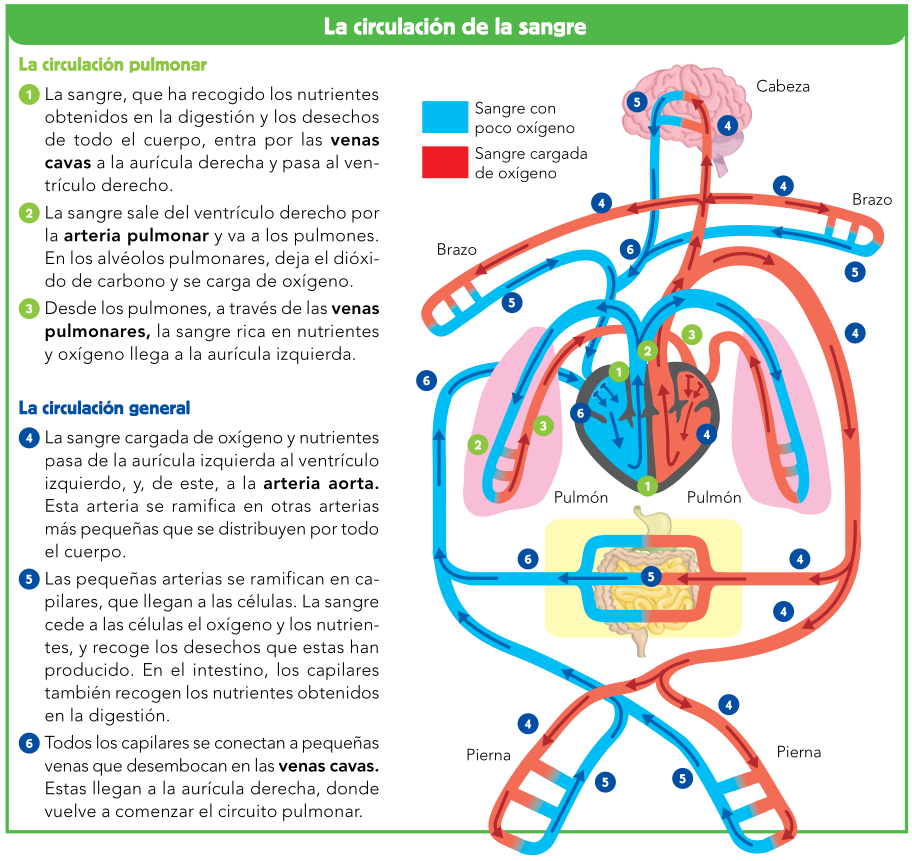
\includegraphics[width=1\linewidth]{Tema3/08_Circulacion.png}
    \caption{La circulación de la sangre}
    \label{fig:circulacion}
\end{figure}

\subsection{La excreción}

La \textbf{excreción} es la expulsión al exterior del cuerpo de las sustancias de desecho que se producen en las 
células.

\vspace{3mm}
Además del dióxido de carbono, que se expulsa mediante el aparato respiratorio, las células producen otras muchas sustancias de desecho, que expulsamos, en su mayor parte, a través del \textbf{aparato excretor} y mediante las \textbf{glándulas sudoríparas} de la piel.

\subsubsection{El aparato excretor}

El aparato excretor (Figura \ref{fig:aparato-excretor}) lo forman los riñones y las vías urinarias.

\begin{itemize}
    \item Los \textbf{riñones}. Son dos órganos con forma de judía, situados en la zona lumbar. Contienen miles de finísimos tubos en los que se limpia la sangre de las sustancias de desecho y se forma la orina.
    \item Las \textbf{vías urinarias}. Son los conductos por los que la orina circula, se almacena y se expulsa al exterior. Son los uréteres, la vejiga urinaria y la uretra.
\end{itemize}

\begin{figure}[!ht]
    \centering
    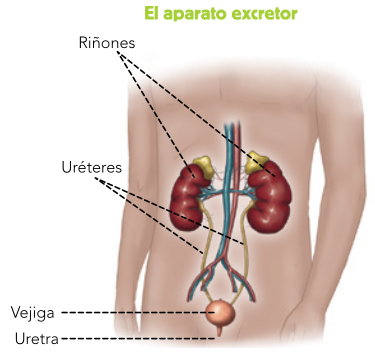
\includegraphics[width=0.7\linewidth]{Tema3/09_Aparato_excretor.png}
    \caption{Aparato excretor}
    \label{fig:aparato-excretor}
\end{figure}

\begin{figure}[!ht]
    \centering
    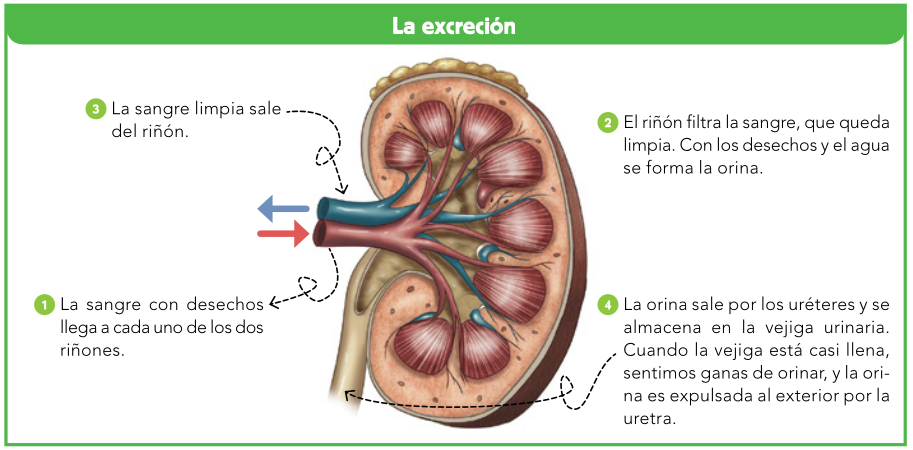
\includegraphics[width=1\linewidth]{Tema3/10_Excrecion.png}
    \caption{La excreción}
    \label{fig:excrecion}
\end{figure}

\subsection{La salud y la emfermedad}

\subsubsection{Qué son la salud y la enfermedad}

La \textbf{salud} es el estado de bienestar desde un punto de vista físico, mental y social. Cuando tenemos salud, nuestro cuerpo funciona bien y nos sentimos a gusto con lo que hacemos, con nuestro ambiente y con los demás.

\vspace{3mm}
La \textbf{enfermedad} es cualquier situación en la que nuestra salud se altera durante un tiempo. Recuerda que una enfermedad se manifiesta con síntomas, que son las señales de que algo no funciona bien en nuestro organismo. Estos síntomas son muy variados y, a partir de ellos, pueden identificarse las enfermedades que podemos sufrir.

\subsubsection{Tipos de enfermedades}

Dependiendo de qué las produce, las enfermedades se pueden clasificar en dos tipos:

\begin{itemize}
    \item Las \textbf{enfermedades infecciosas}. Son las producidas por seres microscópicos, como bacterias o virus, que entran en nuestro cuerpo y nos perjudican. Estos seres llegan a nuestro organismo de varias formas: a través de heridas, picaduras, por el aire que respiramos, por la boca al tomar alimentos en mal estado o sin lavar, al comer con las manos sucias, o al compartir vasos con personas que padecen enfermedades infecciosas… Son enfermedades infecciosas los resfriados, la varicela, la gripe, etc.
    \item Las \textbf{enfermedades no infecciosas}. Son las que se producen por otras causas distintas de los microbios. Por ejemplo: la obesidad, que puede estar provocada por una mala alimentación; las originadas por accidentes, como los cortes, las roturas de huesos, etc.; las causadas por sustancias tóxicas (intoxicaciones); el agotamiento físico y mental provocado por descansar y dormir poco.
\end{itemize}

\subsubsection{Nutrición y salud}

Prevenir es aplicar medidas y hábitos saludables que disminuyen el riesgo de padecer ciertas enfermedades. La prevención se consigue llevando una serie de \textbf{hábitos saludables} para cuidar nuestro organismo. También, acudiendo a \textbf{revisiones médicas} cada cierto tiempo, para detectar si algo funciona mal en nuestro cuerpo y tratarlo antes de que la enfermedad se haga más grave.

\vspace{3mm}
\textbf{Hábitos saludables y nutrición}

\vspace{3mm}
Muchas enfermedades que afectan a los aparatos que intervienen en la nutrición pueden prevenirse siguiendo una serie de hábitos saludables relacionados con el estilo de vida.

\vspace{3mm}
\textbf{Cómo cuidar el aparato digestivo}

\begin{itemize}
    \item Llevar una \textbf{dieta equilibrada} para disminuir el riesgo de enfermedades nutricionales.
    \item \textbf{Tomar fruta y verdura} cada día e incluir en la dieta alimentos que contengan fibra, ya que favorecen el tránsito intestinal.
    \item \textbf{Comer despacio}, masticando bien los alimentos, y tratar de hacer \textbf{cuatro o cinco comidas al día}, preferentemente a las mismas horas.
    \item \textbf{No comer más de lo necesario}, para que tus digestiones sean ligeras.
    \item \textbf{Lavar los alimentos} que tomamos \textbf{y las manos antes y después de comer}, para evitar enfermedades infecciosas e intoxicaciones.
    \item \textbf{Moderar el consumo} de la sal, el chocolate, las salsas picantes, el café, etc., que pueden dañar el aparato digestivo.
    \item Mantener una buena higiene dental lavándote los dientes después de cada comida, para evitar la caries dental.
\end{itemize}

\textbf{Cómo cuidar el aparato respiratorio}

\begin{itemize}
    \item Tratar siempre de \textbf{respirar por la nariz} y no por la boca, ya que las fosas nasales retienen las partículas de polvo, y calientan y humedecen el aire antes de entrar en los pulmones.
    \item Hacer \textbf{ejercicio físico cada día}, ya que mejora la ventilación de los pulmones.
    \item \textbf{No fumar}, ya que el consumo de tabaco se relaciona con muchas enfermedades, entre ellas el cáncer de pulmón.
    \item \textbf{Evitar ambientes contaminados}, y con mucho humo que pueden perjudicar a tus pulmones.
    \item \textbf{Practicar ejercicios de respiración} ya que, además de mejorar la oxigenación de nuestro cuerpo, pueden servir como forma de relajación en situaciones estresantes.
\end{itemize}

\textbf{Cómo cuidar el aparato circulatorio}

\begin{itemize}
    \item Llevar una \textbf{dieta equilibrada} y no abusar de las grasas, la bollería industrial y las golosinas, para evitar enfermedades cardiovasculares.
    \item Realizar \textbf{ejercicio físico a diario y evitar el sedentarismo} para prevenir la obesidad y los infartos.
    \item \textbf{Descansar y dormir} entre 8 y 10 horas son indispensables para evitar la fatiga y el cansancio.
    \item \textbf{Evitar el consumo de alcohol y de tabaco}, para evitar el riesgo de sufrir enfermedades cardiovasculares como los infartos.
\end{itemize}

\textbf{Cómo cuidar el aparato excretor}

\begin{itemize}
    \item \textbf{Beber abundante líquido}, preferiblemente agua, para evitar la concentración de la orina y la aparición de cálculos (piedras en los riñones o en la vejiga).
    \item Llevar una \textbf{dieta equilibrada}, sin abusar de alimentos salados que podrían dañar tus riñones.
\end{itemize}